\subsection{Arquitetura}


%
% Simple topology
%
\begin{frame}\frametitle{Topologia simples}

	\begin{figure}[h]
        \centering
        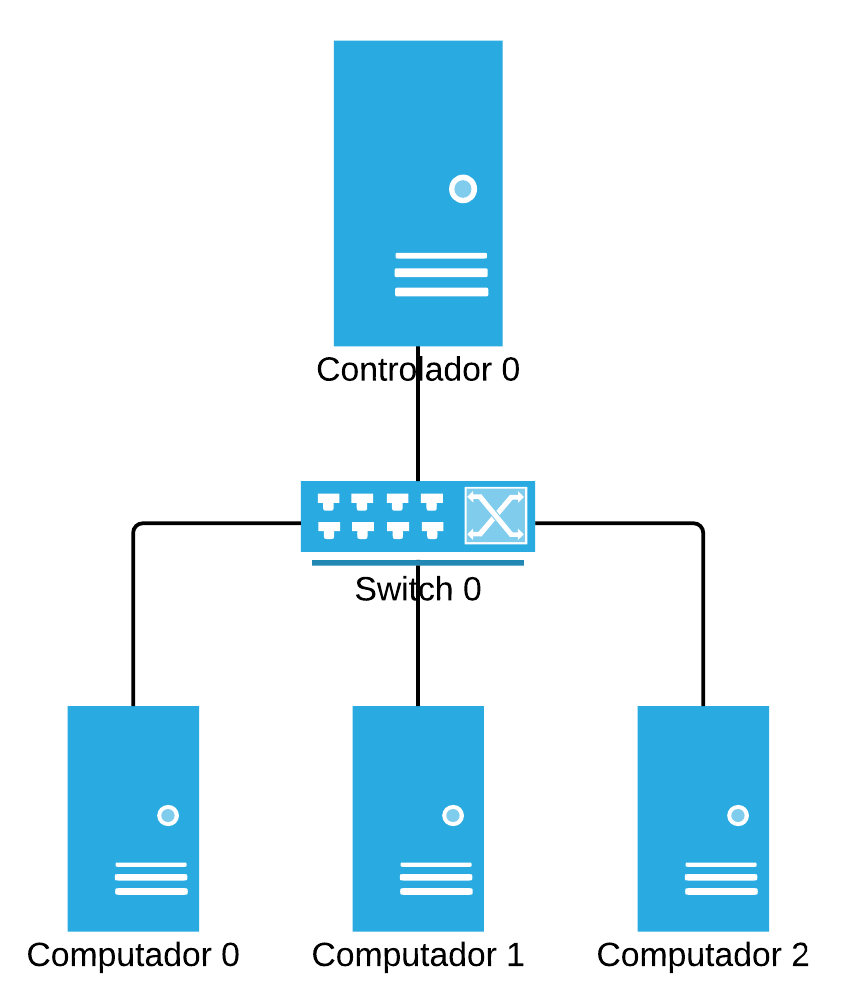
\includegraphics[scale=.8]{images/simple-topology}
    \end{figure}
\end{frame}


%
% N openflow 
%
\begin{frame}\frametitle{Um controlador para \emph{n} comutadores}

	\begin{figure}[h]
        \centering
        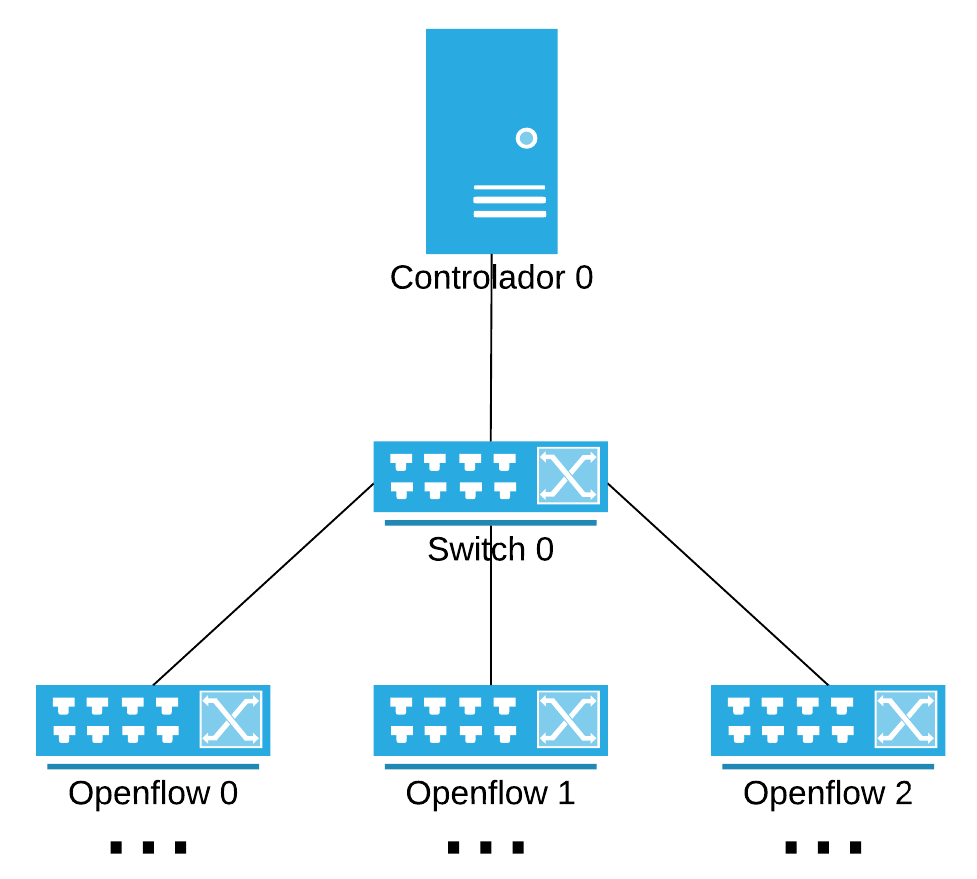
\includegraphics[scale=.8]{images/controller-n-switches}
    \end{figure}
\end{frame}


%
% N to N
%
\begin{frame}\frametitle{\emph{n} controladores para \emph{n} comutadores}

	\begin{figure}[h]\hspace*{-1cm}
        \centering
        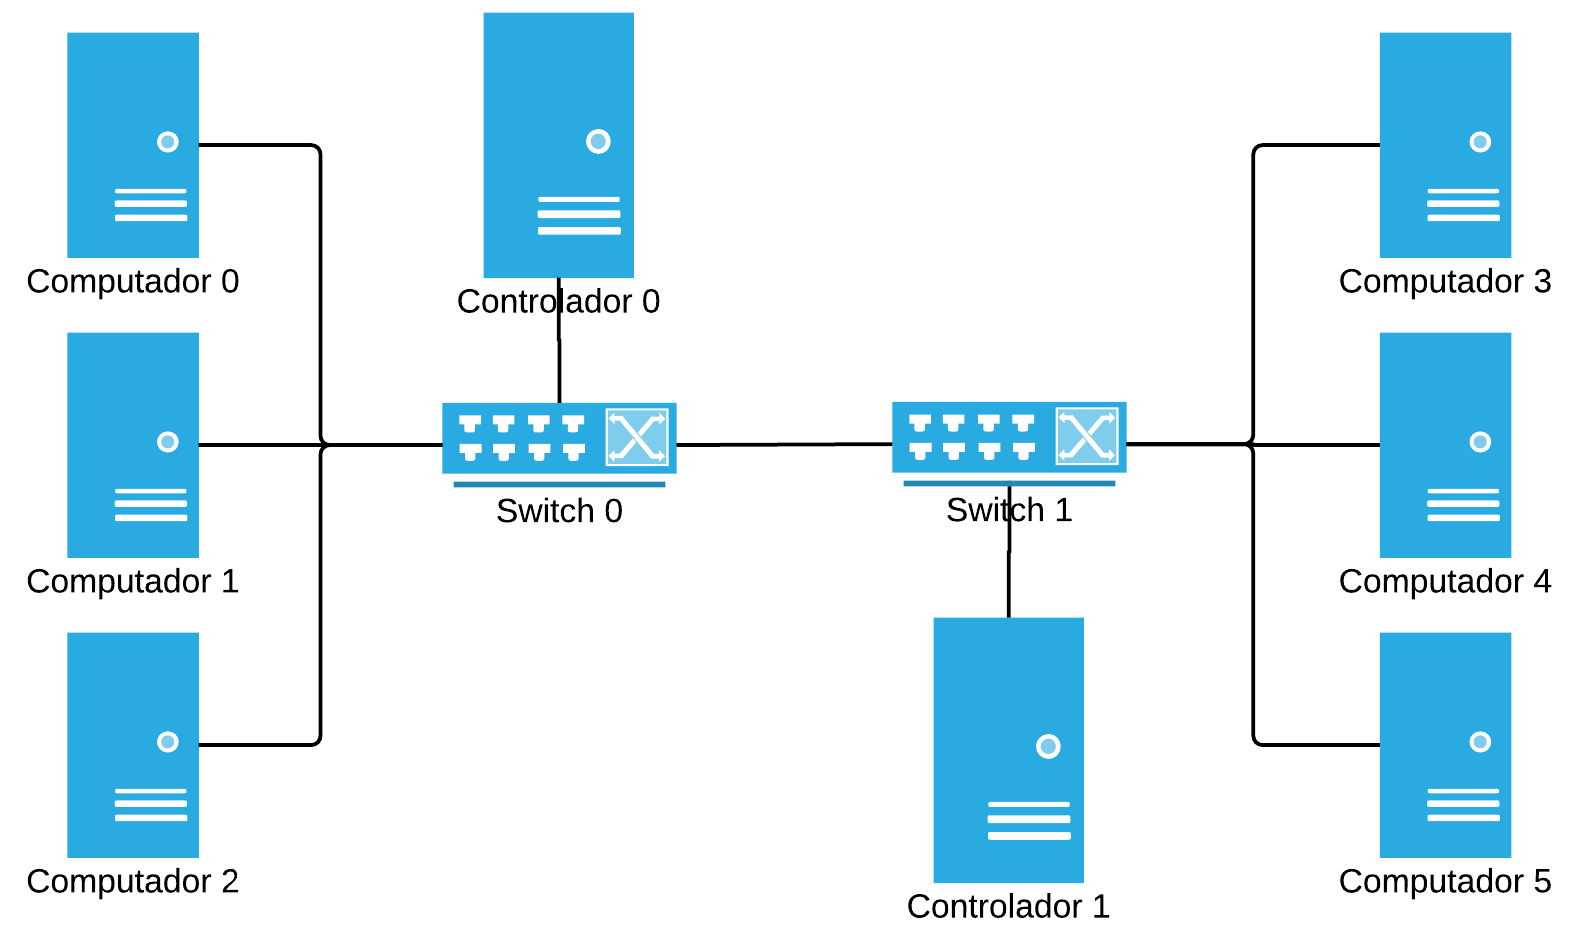
\includegraphics[scale=.8]{images/n-controllers-n-switches}
    \end{figure}
\end{frame}



%
% Distributed openflow controller
%
\begin{frame}\frametitle{Controladores distribuídos}

	\begin{figure}[h]
        \centering
        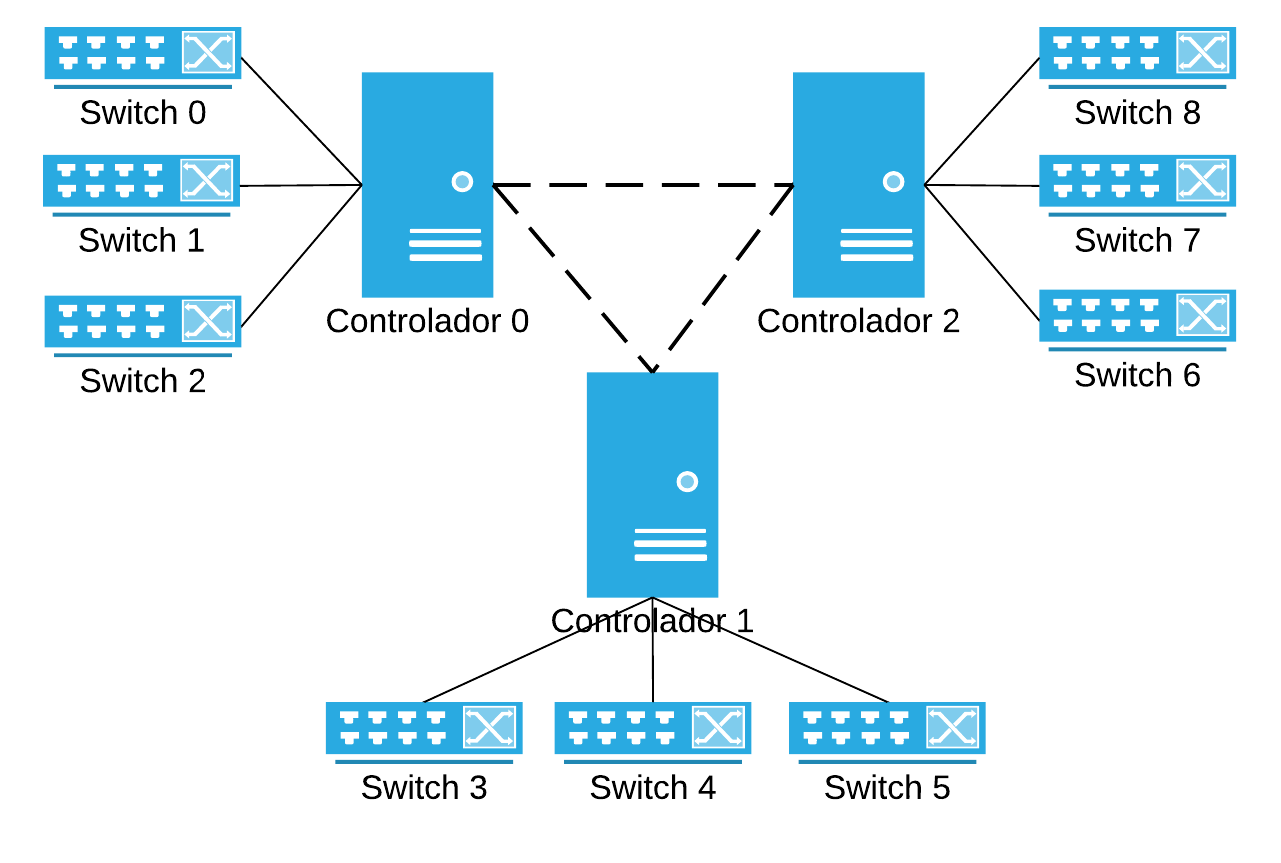
\includegraphics[scale=.9]{images/distributed_sdn_controller}
    \end{figure}
\end{frame}


%
% SDN for Internet architecture
%
\begin{frame}\frametitle{Arquitetura para a Internet}

	\begin{figure}[h]
        \centering
        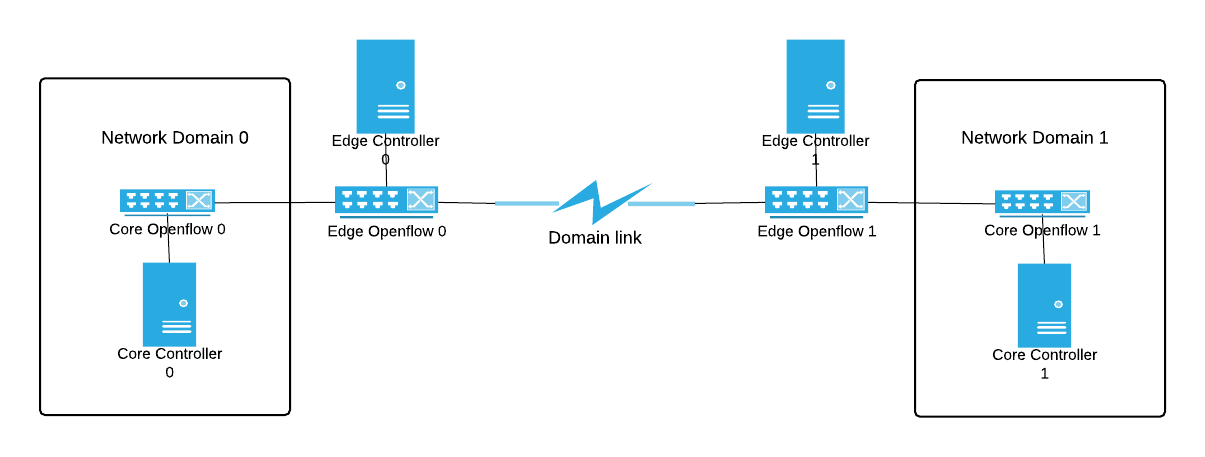
\includegraphics[scale=.6]{images/edge-core-sdn}
    \end{figure}
\end{frame}
